\documentclass[bibliography=totoc,12pt,a4paper]{scrartcl}
\usepackage{amsmath, amssymb, amsthm}
\usepackage{enumerate}% schicke Nummerierung
\usepackage{graphicx}
\usepackage[english, ngerman]{babel}
\usepackage[T1]{fontenc}
\usepackage{lmodern}
\usepackage[utf8]{inputenc}
\usepackage{bigdelim}
\usepackage{multirow}
\usepackage{dsfont}
\usepackage[colorlinks=true,linkcolor=black, citecolor=black]{hyperref}
\usepackage{cite}
\usepackage[nottoc]{tocbibind}
\usepackage{empheq}
\usepackage{fancyhdr}
\usepackage{geometry}
\usepackage{lipsum}
\usepackage{tikz,pgfplots}
\usepackage{nicefrac}
\usepackage{graphicx}
\usepackage{subcaption}
\usetikzlibrary{shapes.misc}
\usetikzlibrary{matrix}
\geometry{a4paper,left=40mm,right=30mm, top=5cm, bottom=5cm} 

\def\@biblabel#1{\textcolor{red}{[#1]}}

\newtheoremstyle{linebreak}   % name
{3pt}                         % Space above
{3pt}                         % Space below
{}                            % Body font
{}                            % Indent amount 1
{\bfseries}                   % Theorem head font
{\newline}                    % Punctuation after theorem head
{.5em}                        % Space after theorem head 2
{}                            % Theorem head spec (can be left empty, meaning ‘normal’)
%\theoremstyle{linebreak}
\newtheoremstyle{exampstyle}
  {\topsep} % Space above
  {\topsep} % Space below
  {} % Body font
  {} % Indent amount
  {\bfseries} % Theorem head font
  {.} % Punctuation after theorem head
  {.5em} % Space after theorem head
  {} % Theorem head spec (can be left empty, meaning `normal')
\theoremstyle{exampstyle}
\newtheorem{defi}{Definition}%[chapter]
\newtheorem{satz}[defi]{Satz}
\newtheorem{theorem}[defi]{Theorem}
\newtheorem{propo}[defi]{Proposition}
\newtheorem{lemma}[defi]{Lemma}
\newtheorem{cor}[defi]{Korollar}
\newtheorem{bem}[defi]{Bemerkung}
\newtheorem{bsp}[defi]{Beispiel}
\newtheorem{folg}[defi]{Folgerung}
%bemerkungen oder Fließtext???
\numberwithin{equation}{section} 
 \newcommand{\newln}{\\&\quad\quad{}}
 \setlength\parindent{0pt}

\renewenvironment{abstract}
 {\small
  \begin{center}
  \bfseries \abstractname\vspace{-.5em}\vspace{0pt}
  \end{center}
  \list{}{%
    \setlength{\leftmargin}{12mm}% <---------- CHANGE HERE
    \setlength{\rightmargin}{\leftmargin}%
  }%
  \item\relax}
 {\endlist}


\usepackage{listings}
\usepackage{color}
 
\definecolor{codegreen}{rgb}{0,0.6,0}
\definecolor{codegray}{rgb}{0.5,0.5,0.5}
\definecolor{codepurple}{rgb}{0.58,0,0.82}
\definecolor{backcolour}{rgb}{0.95,0.95,0.92}
 
\lstdefinestyle{mystyle}{
    backgroundcolor=\color{backcolour},   
    commentstyle=\color{codegreen},
    keywordstyle=\color{magenta},
    numberstyle=\tiny\color{codegray},
    stringstyle=\color{codepurple},
    basicstyle=\footnotesize,
    breakatwhitespace=false,         
    breaklines=true,                 
    captionpos=b,                    
    keepspaces=true,                 
    numbers=left,                    
    numbersep=5pt,                  
    showspaces=false,                
    showstringspaces=false,
    showtabs=false,                  
    tabsize=2
}
 
\lstset{style=mystyle}

\begin{document}

\title{Quasi-Newton Methoden in der Formoptimierung}

\author{Daniel Luft \\ Prof. Dr. V. Schulz}

  \pagestyle{empty}

  % Ab sofort Seitenzahlen in der Kopfzeile anzeigen
  \pagestyle{headings}
  
\selectlanguage{ngerman}

\section{Resultate}
\subsection{???}

\colorbox{red}{l-bfgs springt schnell nahe Lösung: Verwandtschaft zu CG (nocedal + das paper zu konvergenz}
\colorbox{red}{erwähne, dass Gitter Probleme macht; eigentlich Neustart mit Gitter nötig; oder Lameparameter mit Funktion tweaken}
\colorbox{red}{wenn konvergiert, so vllt auch mit lokalen Minima...}
\colorbox{red}{Gitterunabhängig? Ordnung der Bilinearform mit der des Hesseoperators in übereinstimmung? Ausblick biharmonic?}
\colorbox{red}{plotte l-BFGs vs Gradient}
\colorbox{red}{mache Langzeit rechnung mit und ohne Line-search bei Pertubation}
\colorbox{red}{Programme als Wort, Rechtschreibfehler in anderen Chaptern}

Wie angekündigt möchten wir in diesem abschließenden Abschnitt die Resultate aus unserer Programmierung analysieren. Wir haben mehrere Problemgitter und Kombinationen aus Verfahren getestet, und dabei die Daten aufbereitet. \colorbox{red}{Diese Daten werden auf der beigelegten CD samt dem Programm enthalten sein.}
Wir haben uns für die Analyse der Verfahren für zwei Testprobleme entschieden. Zum einen soll ein kleiner Kreis zu einem großen Kreis deformiert werden, wobei die Kreismittelpunkte jeweils gleich bleiben. Somit handelt es sich bei diesem Problem um Deformation einer konvexen Form ohne große Translation. Zum anderen soll ein kleiner Kreis zu einer nierenartigen Form deformiert werden. In diesem Problem findet eine verhätlnismäßig starke Translation statt, außerdem ist die Zielform ein nicht konvex, was dieses Problem deutlich schwieriger macht, als das erste. In beiden Fällen sind die Formen in dem Einheitsquadrat im $\mathbb{R}^2$ eingebettet. Diese sind abgebildet \ref{Meshes}. 
Die Parameter, welche bei der Analyse in betracht kommen, sind als Standard auf folgende Werte gesetzt:
\colorbox{red}{vllt doch die Namen aus dem Program, mit Tabellenverweis}
\begin{align*}
\text{Gitterfeinheit: \hspace{0.2cm} }& 0.1 \text{ (normal)} \hspace{0.65cm} ,0.025 \text{ (fein)} \\
\text{Lamé-Parameter: \hspace{0.2cm} }& 0.0 \text{ (min)} \hspace{1.2cm}  ,30.0 \text{ (max)} \\
\text{Perimeter-Reg.: \hspace{0.2cm} }& 0.00001 \\
\text{Funktionswerte für Zustand: \hspace{0.2cm} }& -10.0 \text{ (außen) },  100.0 \text{ (innen)} \\
\text{Memory-Length: \hspace{0.2cm} }& 60 \\
\text{Toleranz für Ausstieg: \hspace{0.2cm} }& 0.0008 \\
\text{Backtracking: \hspace{0.2cm} }& 5.0 \text{ (start\_scale)}, 0.5 \text{ (shrinkage)}, 0.999 \text{ (c)}
\end{align*}


\newpage
\begin{figure}
	\begin{subfigure}{0.5\textwidth}
	\centering
	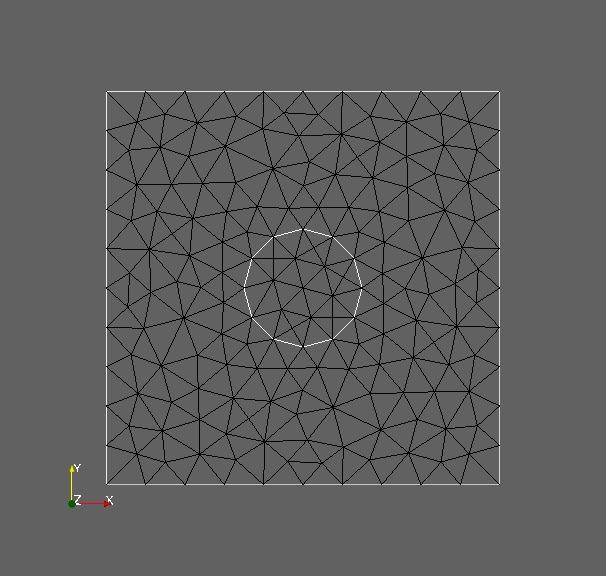
\includegraphics[scale=0.25]{pic_smallcircle.jpg}
	\caption{}	
	\end{subfigure}
	\begin{subfigure}{0.5\textwidth}
	\centering
	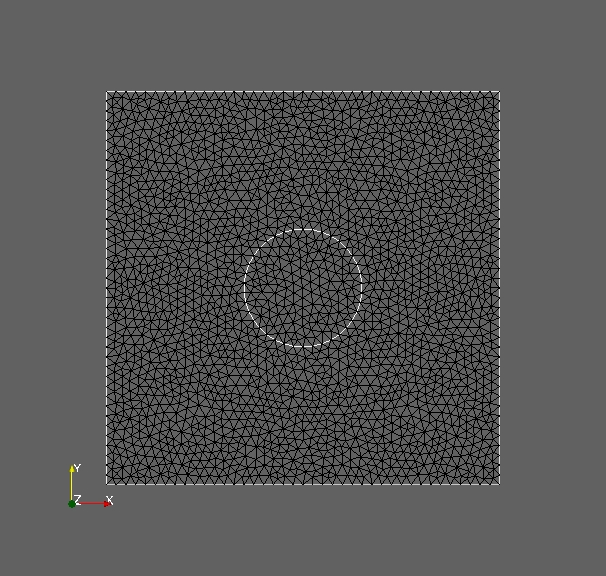
\includegraphics[scale=0.25]{pic_smallcircle_fine.jpg}
	\caption{}	
	\end{subfigure}
	\begin{subfigure}{0.5\textwidth}
	\centering
	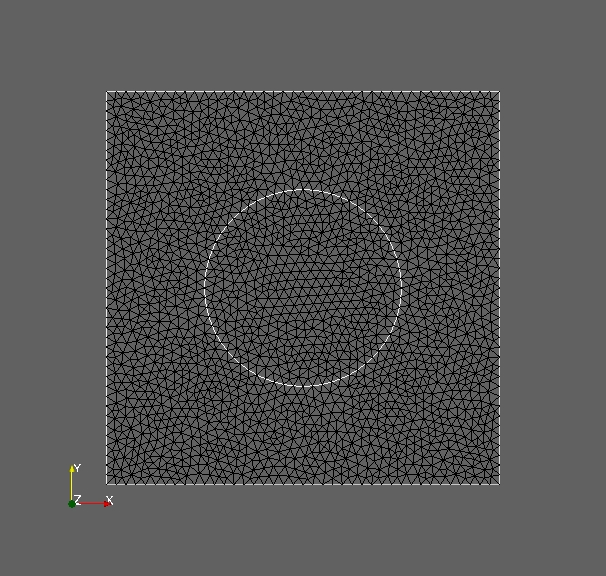
\includegraphics[scale=0.25]{pic_bigcircle_fine.jpg}
	\caption{}	
	\end{subfigure}
	\begin{subfigure}{0.5\textwidth}
	\centering
	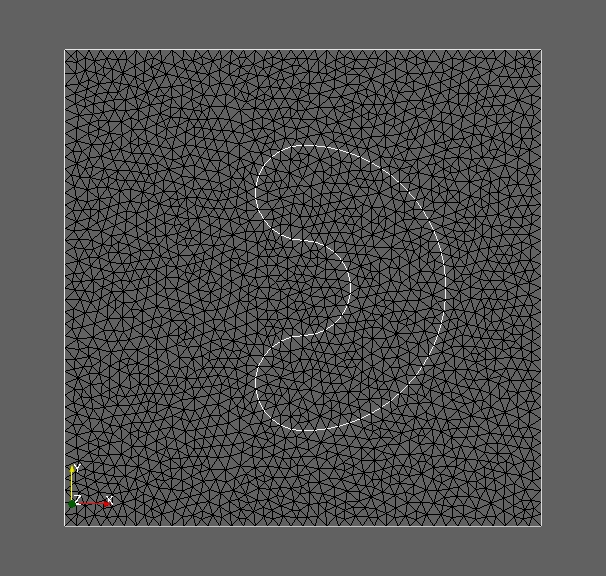
\includegraphics[scale=0.25]{pic_brokendonut_fine.jpg}
	\caption{}	
	\end{subfigure}
\caption{(a) Ausgangsform kleiner Kreis auf grobem Gitter (b) Ausgangsform kleiner Kreis auf feinem Gitter (c) Zielform großer Kreis auf feinem Gitter (d) Zielform broken Donut auf feinem Gitter}
\label{Meshes}
\end{figure}

Wir werden sowohl das L-BFGS-Verfahren, als auch das Gradientenverfahren vergleichen. Außerdem wird jeweils die Linesearch an- und ausgeschaltet, sowie alle oben aufgeführten Parameter, bis auf die Funktionswerte die Zustandsgleichung im Zielgitter, den Verbesserungsfaktor \textsf{c}, und den Skalierungsfaktor \textsf{shrinkage} der Backtracking-Linesearch, variiert. Die Verwendung der Memory-Length von 60 bewirkt, dass es sich in allen folgenden Fällen der Verwendung des L-BFGS-Verfahrens eigentlich um ein BFGS-Verfahren handelt, da die gesamte Historie zur Berechnung der Hesseapproximation benutzt wird. 


Für das Problem der Deformation zum großen Kreis erhalten wir bei dem groben Gitter 
bei Verwendung des Gradientenverfahrens ohne Linesearch Konvergenz nach fast 800 Schritten. Schaltet man das Backtracking ein, so erhält man ebenfalls Konvergenz, jedoch schon bei ca. 450 Schritten. Dies legt nahe, das die Schrittweite durch das anfangliche Hochskalieren der Deformation optimaler wird, der Gradient also der Norm nach relativ klein war. Bei Verfeinerung des Gitters um das 4-fache erhalten wir ebenfalls ohne Verwendung der Linesearch beim Gradientenverfahren Konvergenz nach ca. 650 Schritten. Wieder findet durch Verwendung des Backtracking eine Beschleunigung zur Konvergenz statt, diesmal nach 520 Schritten. Erhöht man das anfangliche Hochskalieren vom Faktor 5 auf 20, so erhält man im feinen Gitter Konvergenz schon nach 120 Schritten. Die Geschwindigkeit zur Konvergenz hat sich also im Vergleich zum Gradientenverfahren ohne Backtracking also um das 5-fache gesteigert, wobei sich die erzeugten Gitter bei Ausstieg des Verfahrens mit oder ohne Linesearch und Veränderung des Hochskalierungsfaktors nicht unterscheiden. 

\colorbox{red}{Plot: feines gitter; no linesearch; linesearch; highstartscale}

Findet das L-BFGS-Verfahren ohne Linesearch Anwendung, so erhält man auf dem groben Gitter keine Konvergenz. Das Verfahren updatet die BFGS-Memory nach mehreren Verletzungen der Curvature Condition nicht, und deformiert das Gebiet schließlich bei Schritt 26 bis zur Unbrauchbarkeit, was in \ref{Destroyedgradient} zu sehen ist. Man beachte die starke Entartung der kaum sichtbaren Zellen kurz vor der Zerstörung des Gitters, welche man im Zoom gut erkennt.


\begin{figure}
	\begin{subfigure}{0.5\textwidth}
	\centering
	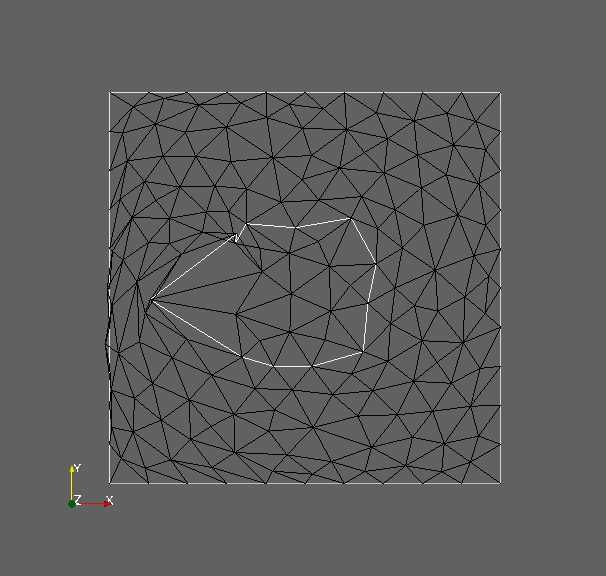
\includegraphics[scale=0.25]{pic_smallcircle_destroyed1.jpg}
	\caption{}	
	\end{subfigure}
	\begin{subfigure}{0.5\textwidth}
	\centering
	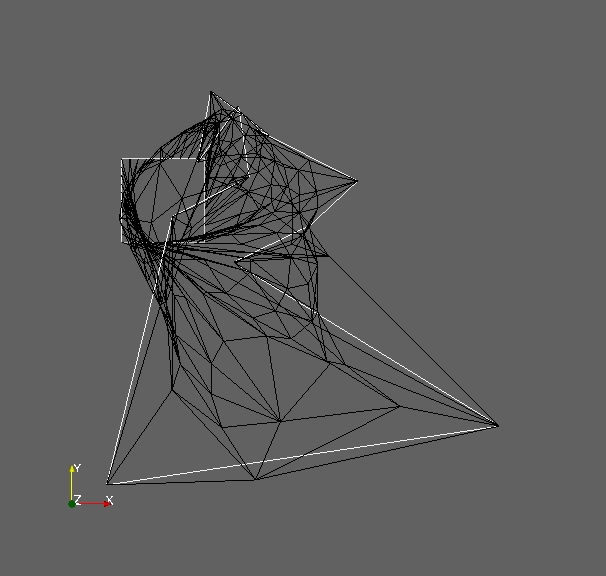
\includegraphics[scale=0.25]{pic_smallcircle_destroyed2.jpg}
	\caption{}	
	\end{subfigure}
\caption{(a) Gitter nach mehrmaligen Schritten unter Verletzung der Curvature Condition und Non-update Schritten (b) der darauf folgende Schritt, Zerstörung des Gitters}
\label{Destroyedgradient}
\end{figure}

Auch bei Verfeinerung des Gitters um das 4-fache erhält man keine Konvergenz des L-BFGS-Verfahrens, sondern erreicht die Zerstörung des Gitters nach Verletzung der Curvature Condition schon im zweiten Schritt, bei der die Form das Einheitsquadrat verlässt. Man beachte, das dieses mal die Richtung des Schrittes in Richtung Optimum geht, jedoch viel zu lang ist, anders als in \ref{Destroyed}, wo zuvor mehrmalige falsche Schritte bei Verletzung der Curvature Condition das Gitter zerstören. Der BFGS-Schritt ist zu sehen in \ref{Destroyedbfgs}. Diese Beobachtung macht erneut deutlich, wie wichtig eine effektive Schrittweitensteuerung bei der Implementierung der Verfahren sind.

\begin{figure}
	\begin{subfigure}{0.5\textwidth}
	\centering
	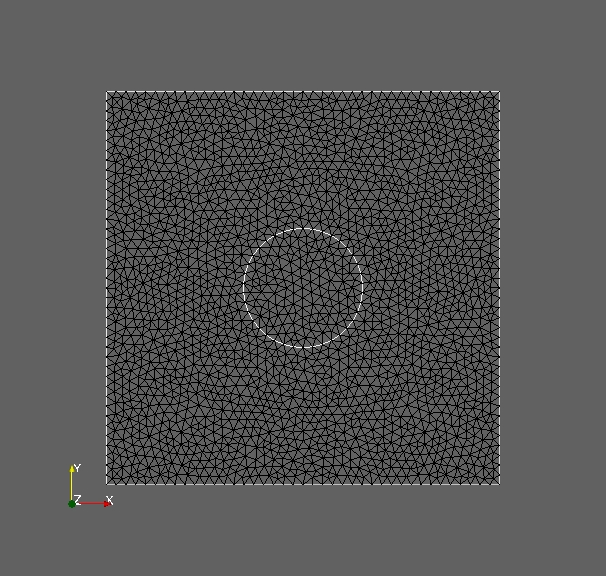
\includegraphics[scale=0.25]{pic_smallcircle_bfgsdestroyed1.jpg}
	\caption{}	
	\end{subfigure}
	\begin{subfigure}{0.5\textwidth}
	\centering
	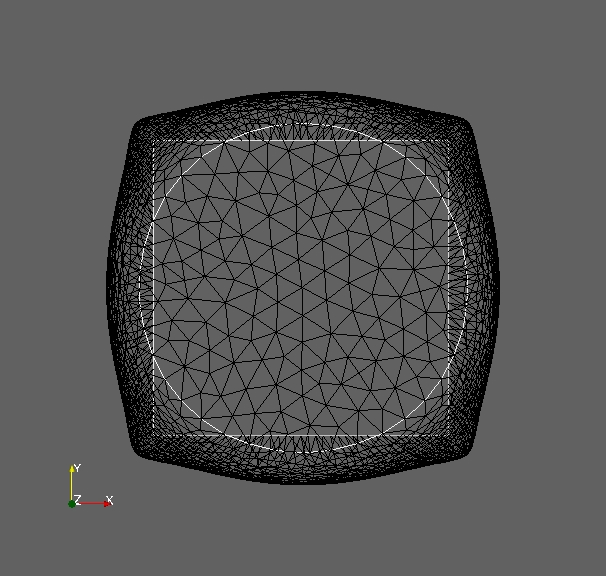
\includegraphics[scale=0.25]{pic_smallcircle_bfgsdestroyed2.jpg}
	\caption{}	
	\end{subfigure}
\caption{(a) 1. Schritt: Gradientenschritt bei feinem Gitter (b) 2. Schritt: BFGS-Schritt mit Entartung des feinen Gitters}
\label{Destroyedbfgs}
\end{figure}

Wir haben auch versucht, die Gitterzerstörung durch Modifikation der lokal variierenden Lamé-Parameter zu begegnen. Alle bisher gezeigten Gitter hatten die Wahl des minimalen Lamé-Parameters von 0. Um zu beobachten, ob die Verfahren instabiler werden, wenn man konstante Lamé-Parameter wählt, haben wir diese konstant auf 30 gesetzt. Man erhält den Output \ref{Destroyedkonstlame}.

\begin{figure}
	\begin{subfigure}{0.3\textwidth}
	\centering
	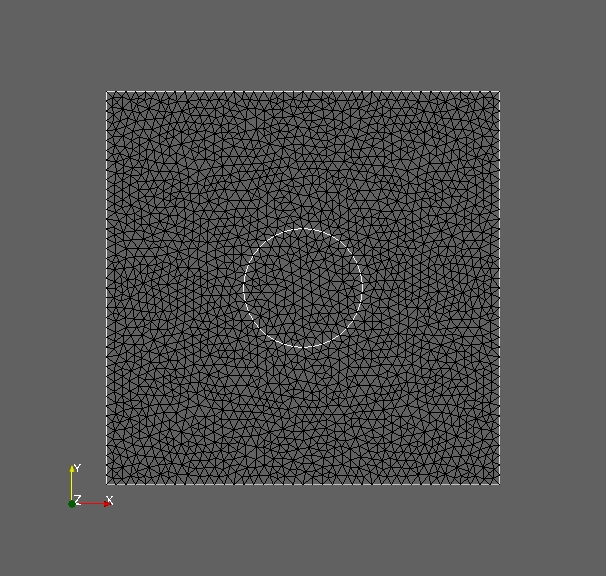
\includegraphics[scale=0.2]{pic_bigcircle_constlame1.jpg}
	\caption{}	
	\centering
	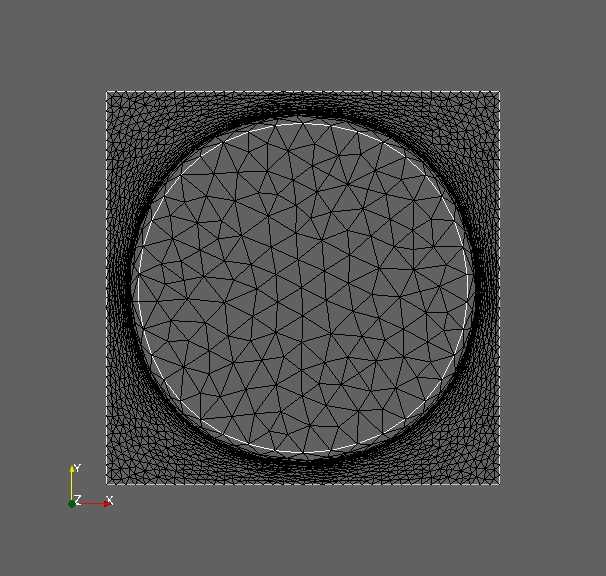
\includegraphics[scale=0.2]{pic_bigcircle_constlame2.jpg}
	\caption{}	
	\end{subfigure}
	\begin{subfigure}{0.3\textwidth}
	\centering
	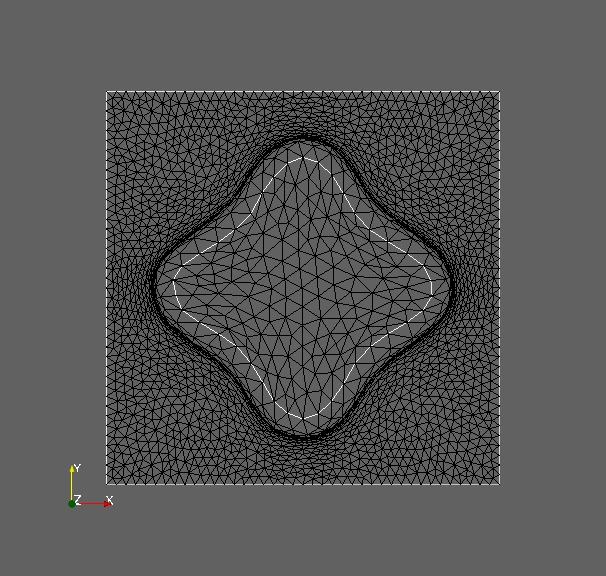
\includegraphics[scale=0.2]{pic_bigcircle_constlame3.jpg}
	\caption{}	
	\centering
	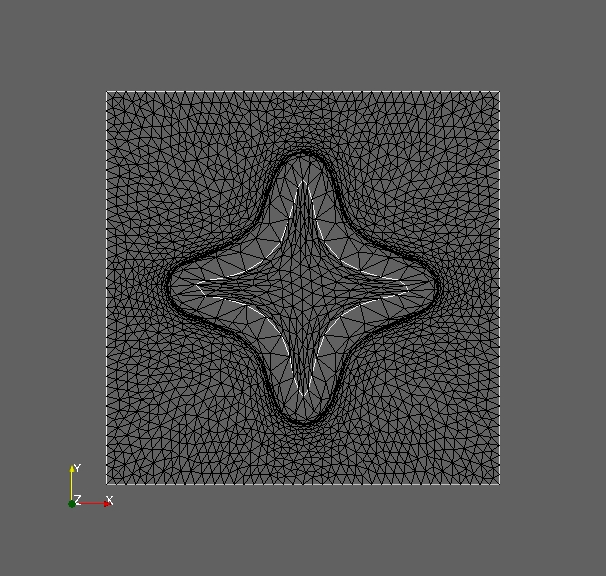
\includegraphics[scale=0.2]{pic_bigcircle_constlame4.jpg}
	\caption{}	
	\end{subfigure}
	\begin{subfigure}{0.3\textwidth}
	\centering
	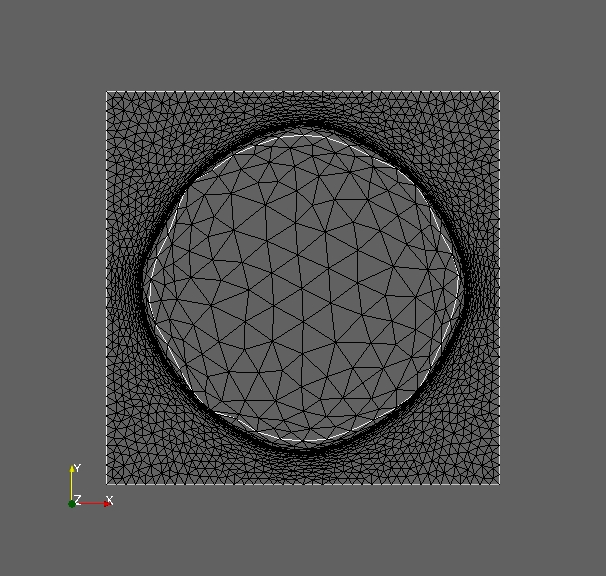
\includegraphics[scale=0.2]{pic_bigcircle_constlame5.jpg}
	\caption{}	
	\centering
	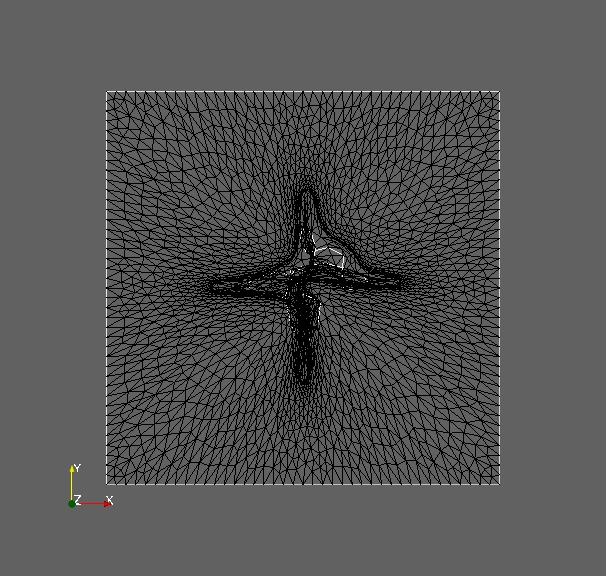
\includegraphics[scale=0.2]{pic_bigcircle_constlame6.jpg}
	\caption{}	
	\end{subfigure}
\caption{BFGS-Verfahren ohne Schrittweitensteuerung bei konstanten Lamé-Parametern mit Wert 30}
\label{Destroyedkonstlame}
\end{figure}

Ein komplett anderes Verhalten stellt sich bei Verwendung der Linesearch ein; in diesem Fall konvergiert das L-BFGS-Verfahren für beide Gitterfeinheiten.

\colorbox{red}{startscale bei bfgs skalierungsunabhängig; bfgs vs lbfgs kein unterschied --> 1 term fehlt; Plot mit Gradient und L-BFGS; zeroed erwähnen; perimeter klein kein unterschied(sogar 0); lok. Min., d.h. kein Abstieg in einem Fall; }

\newpage
\nocite{*}
\bibliographystyle{plain}
\bibliography{papers}

\end{document}
